\documentclass[mathserif]{beamer}

\setbeamertemplate{frametitle}[default][center]%Centers the frame title.
\setbeamertemplate{navigation symbols}{}%Removes navigation symbols.
\setbeamertemplate{footline}{\raisebox{5pt}{\makebox[\paperwidth]{\hfill\makebox[10pt]{\scriptsize\insertframenumber}}}}
\setbeamertemplate{caption}[numbered]

\usepackage{amssymb,amsfonts,amsmath,latexsym,amsthm}
%\usepackage[usenames,dvipsnames]{color}
%\usepackage[]{graphicx}
%\usepackage[space]{grffile}
\usepackage{mathrsfs}   % fancy math font
% \usepackage[font=small,skip=0pt]{caption}
\usepackage[skip=0pt]{caption}
\usepackage{subcaption}
\usepackage{verbatim}
\usepackage{url}
\usepackage{bm}
\usepackage{dsfont}
\usepackage{extarrows}
\usepackage{multirow, bm}
%\input{multi_symbols.tex}


\usepackage{float,bm}
\floatstyle{boxed}
\newfloat{code}{tp}{code}
\floatname{code}{Code Example}
%\input{multi_symbols}
%\usepackage{fontspec}
%\setmainfont{Tahoma}

%\newcommand{\lam}{\lambda}
\newcommand{\bmu}{\bm{\mu}}
\newcommand{\bX}   {\bm{X}}
\newcommand{\bY}   {\bm{Y}}
\newcommand{\bz}   {\bm{z}}
\newcommand{\sig}   {\Sigma}
\newcommand{\bx}{\ensuremath{\mathbf{X}}}
%\newcommand{\X}{\ensuremath{\mathbf{x}}}
%\newcommand{\w}{\ensuremath{\mathbf{w}}}
%\newcommand{\h}{\ensuremath{\mathbf{h}}}
%\newcommand{\V}{\ensuremath{\mathbf{v}}}
%\newcommand{\cov}{\text{Cov}}
\newcommand{\var}{\text{Var}}

\newcommand{\Hrule}{\rule{\linewidth}{0.2pt}}
\newcommand{\argmax}{\mathop{\mathrm{argmax}}}
\newcommand{\argmin}{\mathop{\mathrm{argmin}}}
\newcommand{\minimize}{\mathop{\mathrm{minimize}}}
\def\half{\frac{1}{2}}
\def\th{\mathrm{th}}
\def\sign{\mathrm{sign}}
\def\supp{\mathrm{supp}}
\def\E{\mathrm{E}}
\def\P{\mathrm{P}}
\def\Var{\mathrm{Var}}
\def\Cov{\mathrm{Cov}}
\def\Cor{\mathrm{Cor}}
\def\var{\mathrm{var}}
\def\cov{\mathrm{cov}}
\def\cor{\mathrm{cor}}
\def\rcor{\mathrm{rcor}}
\def\mcor{\mathrm{mcor}}
\def\mCor{\mathrm{mCor}}
\def\dCov{\mathrm{dCov}}
\def\dcov{\mathrm{dcov}}
\def\dVar{\mathrm{dVar}}
\def\dvar{\mathrm{dvar}}
\def\dCor{\mathrm{dCor}}
\def\dcor{\mathrm{dcor}}
\def\trace{\mathrm{trace}}
\def\col{\mathrm{col}}
\def\R{\mathds{R}} 
\def\cA{\mathcal{A}}
\def\cB{\mathcal{B}}
\def\cE{\mathcal{E}}
\def\cF{\mathcal{F}}
\def\cG{\mathcal{G}}
\def\cN{\mathcal{N}}
\def\hbeta{\hat{\beta}}
\def\hy{\hat{y}}
\def\red{\color[rgb]{0.8,0,0}}
\def\white{\color[rgb]{1,1,1}}
\def\blue{\color[rgb]{0,0,0.8}}
\def\green{\color[rgb]{0,0.4,0}}

%\DeclareMathOperator{\var}{Var}
%\DeclareMathOperator{\cov}{Cov}

%\newcommand{\indep}{\rotatebox{90}{\ensuremath{\models}}}
%\newcommand{\notindep}{\not\hspace{-.05in}\indep}

\usepackage{graphicx} %The mode "LaTeX => PDF" allows the following formats: .jpg  .png  .pdf  .mps
\graphicspath{{./PresentationPictures/}} %Where the figures folder is located
\usepackage{listings}
\usepackage{media9}
\usepackage{movie15}
\addmediapath{./Movies/}

\newcommand{\beginbackup}{
   \newcounter{framenumbervorappendix}
   \setcounter{framenumbervorappendix}{\value{framenumber}}
}
\newcommand{\backupend}{
   \addtocounter{framenumbervorappendix}{-\value{framenumber}}
   \addtocounter{framenumber}{\value{framenumbervorappendix}} 
}


%\usepackage{algorithm2e}
\usepackage[ruled,lined]{algorithm2e}
\def\algorithmautorefname{Algorithm}
\SetKwIF{If}{ElseIf}{Else}{if}{then}{else if}{else}{endif}
%\usepackage{times}
%\usepackage[tbtags]{amsmath}
%\usepackage{amssymb}
\usepackage{amsfonts}
%\usepackage{slfortheorems}
\usepackage{epsfig}
\usepackage{graphicx}
%\usepackage[small]{caption}
%\usepackage[square]{natbib}
%\newcommand{\newblock}{}
%\bibpunct{(}{)}{;}{a}{}{,}
%\bibliographystyle{ims}
%\usepackage[letterpaper]{geometry}
%\usepackage{color}
%\setlength{\parindent}{0pt}

\usepackage{natbib}
\bibpunct{(}{)}{;}{a}{}{,}
%\usepackage{hyperref}

\DeclareMathOperator*{\Exp}{Exp}
\DeclareMathOperator*{\TExp}{TExp}
\DeclareMathOperator*{\Bernoulli}{Bernoulli}
\DeclareMathOperator*{\Beta}{Beta}
\DeclareMathOperator*{\Ga}{Gamma}
\DeclareMathOperator*{\TGamma}{TGamma}
\DeclareMathOperator*{\Poisson}{Poisson}
\DeclareMathOperator*{\Binomial}{Binomial}
\DeclareMathOperator*{\NormalGamma}{NormalGamma}
\DeclareMathOperator*{\InvGamma}{InvGamma}
\DeclareMathOperator*{\Cauchy}{Cauchy}
\DeclareMathOperator*{\Uniform}{Uniform}
\DeclareMathOperator*{\Gumbel}{Gumbel}
\DeclareMathOperator*{\Pareto}{Pareto}
\DeclareMathOperator*{\Mono}{Mono}
\DeclareMathOperator*{\Geometric}{Geometric}
\DeclareMathOperator*{\Wishart}{Wishart}

\newcommand{\N}{\mathcal{N}}

%\newcommand{\R}{\mathbb{R}}
\newcommand{\Z}{\mathbb{Z}}
%\newcommand{\E}{\mathbb{E}}
\renewcommand{\Pr}{\mathbb{P}}
\newcommand{\I}{\mathds{1}}
\newcommand{\V}{\mathbb{V}}
\newcommand{\bbeta}{\mathbb{\beta}}

% Math operators
\DeclareMathOperator*{\diag}{diag}
\DeclareMathOperator*{\median}{median}
\DeclareMathOperator*{\Vol}{Vol}

% Miscellaneous commands
\newcommand{\iid}{\stackrel{\mathrm{iid}}{\sim}}
\newcommand{\matrixsmall}[1]{\bigl(\begin{smallmatrix}#1\end{smallmatrix} \bigr)}

\newcommand{\items}[1]{\begin{itemize} #1 \end{itemize}}

\newcommand{\todo}[1]{\emph{\textcolor{red}{(#1)}}}

\newcommand{\branch}[4]{
\left\{
	\begin{array}{ll}
		#1  & \mbox{if } #2 \\
		#3 & \mbox{if } #4
	\end{array}
\right.
}

% approximately proportional to
\def\app#1#2{%
  \mathrel{%
    \setbox0=\hbox{$#1\sim$}%
    \setbox2=\hbox{%
      \rlap{\hbox{$#1\propto$}}%
      \lower1.3\ht0\box0%
    }%
    \raise0.25\ht2\box2%
  }%
}
\def\approxprop{\mathpalette\app\relax}

\newcommand{\btheta}{{\bm\theta}}
\newcommand{\bbtheta}{{\pmb{\bm\theta}}}

%\usepackage{zref-savepos}
%
%\newcounter{restofframe}
%\newsavebox{\restofframebox}
%\newlength{\mylowermargin}
%\setlength{\mylowermargin}{2pt}
%
%\newenvironment{restofframe}{%
%    \par%\centering
%    \stepcounter{restofframe}%
%    \zsavepos{restofframe-\arabic{restofframe}-begin}%
%    \begin{lrbox}{\restofframebox}%
%}{%
%    \end{lrbox}%
%    \setkeys{Gin}{keepaspectratio}%
%    \raisebox{\dimexpr-\height+\ht\strutbox\relax}[0pt][0pt]{%
%    \resizebox*{!}{\dimexpr\zposy{restofframe-\arabic{restofframe}-begin}sp-\zposy{restofframe-\arabic{restofframe}-end}sp-\mylowermargin\relax}%
%        {\usebox{\restofframebox}}%
%    }%
%    \vskip0pt plus 1filll\relax
%    \mbox{\zsavepos{restofframe-\arabic{restofframe}-end}}%
%    \par
%}


\usepackage{tikz}
\usetikzlibrary{arrows}

%\usepackage[usenames,dvipsnames]{xcolor}
\usepackage{tkz-berge}
\usetikzlibrary{fit,shapes}

\usepackage{calc}
%%
%% The tikz package is used for doing the actual drawing.
%\usepackage{tikz}
%%
%% In order to be able to put arrowheads in the middle of directed edges, we need an extra library.
\usetikzlibrary{decorations.markings}
%%
%% The next line says how the "vertex" style of nodes should look: drawn as small circles.
\tikzstyle{vertex}=[circle, draw, inner sep=0pt, minimum size=6pt]
%%
%% Next, we make a \vertex command as a shorthand in place of \node[vertex} to get that style.
\newcommand{\vertex}{\node[vertex]}
%%
%% Finally, we declare a "counter", which is what LaTeX calls an integer variable, for use in
%% the calculations of angles for evenly spacing vertices in circular arrangements.
\newcounter{Angle}

\newtheoremstyle{example}
{\topsep} % space above
{\topsep} % space below
{} % body font
{} % indent
{\bf} % head font
{:} % punctuation between head and body
{0.5em} % space after head
{} % manually specify head
%{\thmname{#1}\thmnumber{ #2}\thmnote{:#3}} % manually specify head

\theoremstyle{example}
\newtheorem{ex}{Example}[section]

\newtheoremstyle{definition}
{\topsep} % space above
{\topsep} % space below
{} % body font
{} % indent
{\sc} % head font
{:} % punctuation between head and body
{0.5em} % space after head
{} % manually specify head
%{\thmname{#1}\thmnumber{ #2}\thmnote{:#3}} % manually specify head

\theoremstyle{definition}
\newtheorem{defn}{Definition}[section]

\theoremstyle{rem}
\newtheorem{rem}{Remark}[section]

\newtheoremstyle{theorem}
{\topsep} % space above
{\topsep} % space below
{} % body font
{} % indent
{\sc} % head font
{:} % punctuation between head and body
{0.5em} % space after head
{} % manually specify head
%{\thmname{#1}\thmnumber{ #2}\thmnote{:#3}} % manually specify head

\theoremstyle{theorm}
\newtheorem{thm}{Theorem}[section]



%%%to add in new counter for slides in beamer

%\setbeamertemplate{footline}{
%  \leavevmode%
%  \hbox{%
%  \begin{beamercolorbox}[wd=.333333\paperwidth,ht=2.25ex,dp=1ex,center]{author in head/foot}%
%    \usebeamerfont{author in head/foot}\insertshortauthor~~(\insertshortinstitute)
%  \end{beamercolorbox}%
%  \begin{beamercolorbox}[wd=.333333\paperwidth,ht=2.25ex,dp=1ex,center]{title in head/foot}%
%    \usebeamerfont{title in head/foot}\insertshorttitle
%  \end{beamercolorbox}%
%  \begin{beamercolorbox}[wd=.333333\paperwidth,ht=2.25ex,dp=1ex,right]{date in head/foot}%
%    \usebeamerfont{date in head/foot}\insertshortdate{}\hspace*{2em}
%    \insertframenumber{} \hspace*{2ex} % hier hat's sich ge�ndert
%  \end{beamercolorbox}}%
%  \vskip0pt%
%}



%%%%%

\newcommand*\oldmacro{}
\let\oldmacro\insertshortauthor
\renewcommand*\insertshortauthor{
  \leftskip=.3cm
\insertframenumber\,/\,\inserttotalframenumber\hfill\oldmacro}




%\excludecomment{notbeamer}
%\includecomment{beamer}



\title{Bayesian Model Selection}
\author{Rebecca C. Steorts \\ Bayesian Methods and Modern Statistics: STA 360/602}
\date{ }

\begin{document}

\maketitle

\frame{
\begin{itemize}
\item Knowledge of linear regression is assumed. 
\item How can we do variable selection?
\item Bayes factors.
\item Gibbs sampling.
\end{itemize}
}

\begin{frame}

\begin{figure}[htbp]
\begin{center}
\includegraphics[width=0.9\textwidth]{linear-regression}
\label{default}
\end{center}
\end{figure}




\end{frame}

\frame{
We assume $\bY$ observations and covariates $\bX$.

\vskip 1em

Recall that $$\bY_{n\times 1} = \bX_{n\times p}\bm{\beta}_{p \times 1}+ \epsilon_{n \times 1}$$

$$\epsilon \stackrel{}{\sim} N(0, \sigma^2 I_n). $$

Recall that $E(\bY\mid \bX)$ is linear in it's parameter values.

\vskip 1 em For a thorough review see Hoff or your notes from STA 521.
}

\frame{
\frametitle{Oxygen uptake}

\begin{itemize}
\item Twelve healthy men that don't exercise recruited to study effects of 2 exercise programs on oxygen uptake
\item Program one: 12 weeks of flat running 
\item Program two: 12 weeks of step aerobics
\end{itemize}



}

\frame{
\frametitle{}
We estimate the coefficients $\hbeta \in \R^p$ by least squares:
$$\hbeta = \argmin_{\beta \in \R^p} \|y-X\hbeta\|_2^2$$
This gives
$$\hbeta = (X^T X)^{-1} X^T y$$
(Check: does this match the expressions for univariate regression,
without and with an intercept?)

\bigskip
The fitted values are
$$\hy = X\hbeta = X(X^T X)^{-1} X^T y$$
This is a linear function of $y$, $\hy = Hy$, where
$H=X(X^T X)^{-1} X^T$ is sometimes called the {\red hat matrix}
}

\frame{
Let SSR denote sum of squared residuals. 
$$ \min_\beta SSR(\hbeta) = \min_\beta  \|y-X\hbeta\|_2^2$$
Then 
\begin{align}
 \frac{\partial SSR(\hbeta)}{\partial d\hbeta} &= 
\frac{\partial (y-X\hbeta)^T(y-X\hbeta)}{\partial d\hbeta} \\
&= \frac{\partial \bY^T\bY - 2\hbeta^T\bX^T\bY + \hbeta^T\bX^T\bX\hbeta}{\partial d\hbeta}\\
& = -  2\bX^T\bY + 2\bX^T\bX\hbeta
\end{align}
This implies $-  \bX^T\bY + \bX^T\bX\hbeta= 0 \implies \hbeta  = (\bX^T\bX)^{-1}\bX^T\bY. $
\vskip 1em
Called the ordinary least squares estimator. When is it unique?
}

\frame{
$$\hbeta  = (\bX^T\bX)^{-1}\bX^T\bY. $$
\vskip 1em
$$E(\hbeta ) = \bbeta.$$
\vskip 1em
\begin{align}
\Var(\hbeta) &= \Var\{ (\bX^T\bX)^{-1}\bX^T\bY\}\\
 &=
(\bX^T\bX)^{-1}\bX^T \sigma^2 I_n \bX (\bX^T\bX)^{-1}\\
& = \sigma^2  (\bX^T\bX)^{-1}
\end{align}

$$\hbeta \sim MVN(\bbeta, \sigma^2  (\bX^T\bX)^{-1}).$$

}

\frame{

Suppose
\begin{align}
\bY \mid \bX, \bm{\beta}, \sigma^2 &\sim MVN(\bX\bm{\beta}, \sigma^2 I)\\
\bbeta &\sim MVN(\bbeta_o, \Sigma_o)
\end{align}

What is the form of the distribution of $\bbeta \mid \bY, \bX, \sigma^2$?

Recall it's $MVN(\mu_n, \Sigma_n)$
\vskip 1em
Let's think about the covariance first. 
$$\Sigma_n = [\Sigma_o ^{-1}+\bX^T\bX\sigma^2]^{-1}.$$
Now let's think about the mean. 
$$\mu_n = [\Sigma_o ^{-1}+X^TX\sigma^2]^{-1}(\bX^T\bY/\sigma^2 + \Sigma_o^{-1} \bbeta_o)$$


}

\frame{
Suppose we don't know $\sigma^2.$\\
Let $\gamma = 1/\sigma^2.$
\begin{align}
\bY \mid \bX, \bm{\beta}, \sigma^2 &\sim MVN(\bX\bm{\beta}, \sigma^2 I)\\
\bbeta &\sim MVN(\bbeta_o, \Sigma_o)\\
\gamma &\sim IG(\nu_o/2,\nu_o\sigma_o^2/2).
\end{align}
}

\frame{
Then
\begin{align}
&p(\gamma \mid \bY, \bX, \bbeta)\\
& = p(\gamma) p(\bY \mid bX,  \bY, \bbeta)\\
& \propto \gamma^{(\nu_o +n)/2-1}\exp\{
-\gamma \times \nu_o \sigma_o^2/2
\}\\
& \qquad \times
\gamma^{n/2}\exp\{-\gamma \times SSR(\bbeta)/2
\} \\
& \propto \gamma^{{(\nu_o + n)/2  -1}}
\exp\{-\gamma
(
\nu_o \sigma_o^2/2 + SSR(\bbeta)/2
)
\}
\end{align}
Thus, $$\gamma \mid \bY, \bX, \bbeta \sim IG((\nu_o + n)/2,(\nu_o \sigma_o^2/2 + SSR(\bbeta))/2
)$$

}

\frame{

In order to update $p(\bbeta, \sigma^2 \mid \bY, \bX)$ sample through a two-stage Gibbs sampler. 

\vskip 1em

This is similar to other examples before, and the details can be found in Hoff. (Cycle through the MVN and the IG). 



}

\frame{
\frametitle{Model selection}

\begin{itemize}
\item Often we have a large number of covariates.
\item Using all of them induces poor statistical performance.
\item How can we reduce the covariates and have good inference and prediction?
\item Common method: Backwards and stepwise regression (slow). 
\end{itemize}
}

\frame{
\frametitle{Bayesian model comparison}

Suppose that we believe some of the regression coefficients are 0. 
\vskip 1em
Come up with a prior distribution that reflects the probability of this occuring.
\vskip 1em
Consider 
$$y_i = z_1 b_1 x_{i,1} +\ldots  z_p b_p x_{i,p}, $$
where $b_p$ is a real number and $z_j$ indicate which regression coefficients are nonzero.
\vskip 1em
Note: $\beta_j = b_j \times z_j.$


}


\frame{
Bayesian model selection works by obtaining a posterior distribution for $\bz.$
\vskip 1em
Assume a prior $p(\bz)$. 
\vskip 1em
Then $$p(\bz \mid \bY, \bX) = \frac{p(\bz) p(\bY\mid \bX, \bz)}{\sum_z p(\bz) p(\bY\mid \bX, \bz)}$$

}

\frame{
Suppose we want to compare two models $z_a$  and $z_b$ . 
Consider $$\text{odds}(z_a,z_b\mid \bY, \bX) = \frac{p(z_a\mid \bY, \bX)}{p(z_b\mid \bY, \bX)}
= \frac{p(z_a)}{p(z_b)} \times \frac{p(\bY\mid \bX, z_a)}{p(\bY\mid \bX, z_b)}$$

This is posterior odds = prior odds $\times$ ``Bayes factor"

\vskip 1em

``Bayes factor": how much the data favor model $z_a$ over model $z_b$

\vskip 1em

To obtain a posterior distribution over models, we must compute $p(\bY \mid \bX, \bz)$ for \emph{each} model under consideration.


}

\frame{
We must compute 
\begin{align}
p(\bY \mid \bX, \bz) &= \int \int p(\bY, \bbeta, \sigma^2, \mid \bX, \bz) \\
&\int \int p(\bY \mid \bX, \bz)p(\bbeta \mid \bX, \bz) p(\sigma^2).
\end{align}
To do the \emph{least amount of calculus}, we can put a \emph{g-prior} on
$\bbeta$

$$ \bbeta \mid \bX, \bz \sim MVN(0, g\; \sigma^2 (\bX^T\bX)^{-1}).$$

}

\frame{
\frametitle{What is a g-prior?}
(Hoff, Section 9.2, p. 156-157). 
Based upon the prior should be invariant to changes in the scale of the covariates. 
\begin{itemize}
\item Defined $\tilde{\bX} = H\bX$ for some matrix $H.$
\item Suppose we obtain a posterior of $\bbeta$ from $\bY$ and $\bX.$
\item According to the idea of invariance above, then the posterior of $\bbeta$
and $H\bbeta$ should be the same.
\item Homework: Condition is met if $\beta_o = 0$ and $\Sigma_o = k (\bX^T\bX)^{-1}$ for $k>0.$
\end{itemize}

Popular choice: let $k = g\sigma^2$ for $g>0.$ This is the g-prior.
}

\frame{

Given the g-prior $$ \bbeta \mid \bX, \bz \sim MVN(0, g\; \sigma^2 (\bX^T\bX)^{-1}),$$
$p(\bY \mid \bX, \bz) $
can be worked out in closed form (details p. 165). 
\vskip 1em
Go through the details on your own. 
}
\frame{
This results in being able to compute
\begin{align}
\frac{p(\bY \mid \bX, \bz_a) }{p(\bY \mid \bX, \bz_b) }
& =
(1 + n)^{(p_{z_b} - p_{z_a})/2}
\times \left( \frac{
s_{z_a}^2}{s_{z_b}^2 } \right)^{1/2}\\
&\times
\left(\frac{s_{z_b}^2 + SSR_{g}^{{z_b}}
}
{s_{z_b}^2 + SSR_{g}^{{z_a}}}
\right)^{(n+1)/2}
\end{align}

We have a ratio of the marginal probabilities, giving us a balance between model complexity and model fit. 
\vskip 1em
 Suppose $p_{z_b}$ is large compared to $p_{z_a}.$
\vskip 1em
This causes a penalization of model $z_b$
\vskip 1em
Note that a large value of $SSR_{g}^{{z_b}}$ compared to $SSR_{g}^{{z_a}}$ will penalize model $z_a$.

}

\frame{

\begin{figure}[htbp]
\begin{center}
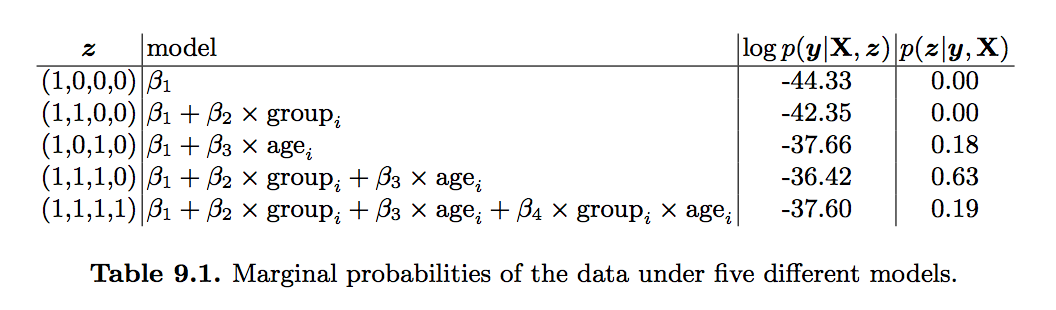
\includegraphics[width=0.8\textwidth]{table91}
\caption{The most probable model is the one corresponding $\bz = (1,1,1,0)$}
\label{default}
\end{center}
\end{figure}


}

\frame{
\center
What is the biggest downside of this approach?

}

\frame{

How do we fix it easily using what we've learned so far in the course? 

}

\frame{

Suppose $p$ is large. Then $2^p$ models to consider. 
\vskip 1em
Instead let's use a Gibbs sampler to search through the space of models for values where $\bz$ has a high posterior probability. 
\vskip 1em
Generate a new value of $\bz$ via $$p(z_j \mid \bY, \bX, \bz_{-j}).$$
\vskip 1em
The full conditional that $z_j=1$ can be written as $o_j/(o_j +1).$
\begin{align}
o_j &= \frac{ p(z_j = 1 \mid \bY, \bX, \bz_{-j})}
{p(z_j = 0 \mid \bY, \bX, \bz_{-j})} \\
&=
\frac{ p(z_j = 1 ) p(\bY \mid \bX, \bz_{-j}, z_j=1) }
{p(z_j = 0) p(\bY \mid \bX, \bz_{-j}, z_j=0)}
\end{align}
}

\frame{
Note: we may also want to obtain posterior samples of $\bbeta$ and $\sigma^2.$
\vskip 1em
Using the conditional distributions from Section 9.2, we can sample from these directly. 
\vskip 1em
The Gibbs sampling scheme requires using Section 9.2 and 9.3 (covered in lab).
}

\frame{

\begin{figure}[htbp]
\begin{center}
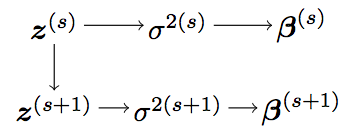
\includegraphics[width=0.4\textwidth]{gibbs-alg}
\caption{Start with $\bz^{(s)}.$ Then in random order update $z_j$ from its full conditional. }
\label{default}
\end{center}
\end{figure}
}
\frame{
Generate $$\{ \bz^{(s+1)}, \sigma^{2(s+1)}, \bbeta^{(s+1)} \}:$$
\begin{enumerate}
\item Set $\bz = \bz^{(s)}$
\item For $j \in \{1,\ldots, p\}$ in random order, replace $z_j$ with a sample from 
$$p(z_j \mid \bz_{-j}, \bY, \bX)$$
\item Set $\bz^{(s+1)} = \bz^{(s)}$
\item Sample $\sigma^{2(s)} \sim p(\sigma^2 \mid \bz^{(s+1)}, \bY, \bX)$
\item Sample $\bbeta^{(s+1)} \sim p(\bbeta \mid \bz^{(s+1)}, \sigma^{2(s+1)}, \bY, \bX)$
\end{enumerate}


}

\frame{

Lab this week: Linear regression and understanding model selection using the diabetes data.


}

\end{document}